\iffalse
                       
                        
                        
                        
                    
                        \author{AI24BTECH11006 - Bugada Roopansha}
                        \section{ae}
                        \chapter{2014}
                        \fi
 
    \item A structural member of rectangular cross-section $10 \text{ mm} \times 6 \text{ mm}$ and length $1 \text{ m}$ is made of steel $\brak{\text{Young's modulus is } 200 \text{ GPa}}$ $\brak{\text{coefficient of thermal expansion is } 12 \times 10^{-6}/^{\circ}\text{C}}$. It is rigidly fixed at both ends and then subjected to a gradual increase in temperature. Ignoring the three-dimensional effects, the structural member will buckle if the temperature is increased by $\Delta T$ \degree C, which is
	   \centering
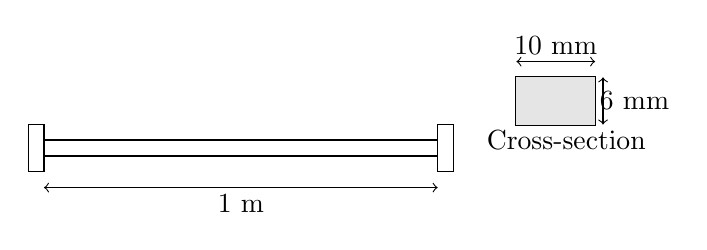
\begin{tikzpicture}
    % Draw the main beam
    \draw[thick] (0,0) -- (5,0);
    \draw[thick] (0,-0.2) -- (5,-0.2);
    
    % Add end supports
    \draw (-0.2,-0.4) rectangle (0,0.2);
    \draw (5,-0.4) rectangle (5.2,0.2);
    
    % Add dimension line and label
    \draw[<->] (0,-0.6) -- (5,-0.6);
    \node at (2.5,-0.8) {1 m};

    % Cross-section view
    \draw[thick] (6,0.2) rectangle (7,0.8);
    \fill[gray!20] (6,0.2) rectangle (7,0.8);
    
    % Cross-section labels
    \draw[<->] (7.1,0.2) -- (7.1,0.8);
    \node at (7.5,0.5) {6 mm};
    \draw[<->] (6,1) -- (7,1);
    \node at (6.5,1.2) {10 mm};
    
    % Add Cross-section text
    \node[anchor=west] at (5.5,0) {Cross-section};

\end{tikzpicture}






	    \begin{enumerate}
        \item $19.74$
        \item $9.87$
        \item $78.96$
        \item $39.48$
    \end{enumerate}


    \item A gas cylinder \brak{\text{closed thin-walled cylindrical pressure vessel}} of diameter $30 \text{ cm}$ and wall thickness $1 \text{ mm}$ is subjected to a design maximum internal pressure of $5 \text{ bar}$ $\brak{0.5 \text{ MPa}}$. The material used for manufacturing this cylinder has a failure stress of $260 \text{ MPa}$. Assuming von Mises failure criterion, the factor of safety \brak{\text{with respect to maximum allowable stress}} for this cylinder is
    \begin{enumerate}
        \item $2.8$
        \item $2.0$
        \item $6.9$
        \item $4.0$
    \end{enumerate}

    \item A cantilevered beam is subjected to a parabolic distribution of shear traction at the right edge while the top and bottom surfaces are traction-free. To solve this problem, the following Airy's stress function is proposed: $\phi = C_1 xy + C_2 xy^3 + C_3 x^2 y^2 + C_4 x^3 y$. This is an admissible Airy's function that would satisfy the bi-harmonic equation as well as the boundary conditions if and only if
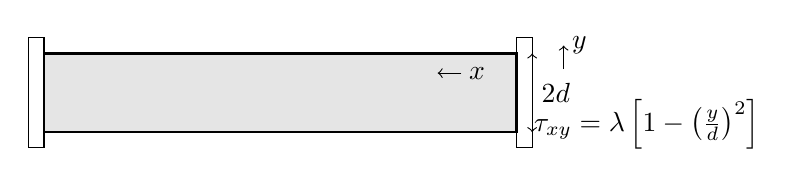
\begin{tikzpicture}
    % Draw the beam
    \fill[gray!20] (0,0) rectangle (6,1);
    \draw[thick] (0,0) rectangle (6,1);
    
    % Add end supports
    \draw (-0.2,-0.2) rectangle (0,1.2);
    \draw (6,-0.2) rectangle (6.2,1.2);
    
    % Dimension line for height
    \draw[<->] (6.2,0) -- (6.2,1);
    \node at (6.5,0.5) {$2d$};
    
    % Label for x-axis
    \node at (5.5,0.75) {$x$};
    \draw[->] (5.3,0.75) -- (5,0.75);
    
    % Label for y-axis
    \node at (6.8,1.1) {$y$};
    \draw[->] (6.6,0.8) -- (6.6,1.1);
    
% Add equation text
    \node[anchor=west] at (6.1,0.1) {$\tau_{xy} = \lambda \left[ 1 - \left( \frac{y}{d} \right)^2 \right]$};
\end{tikzpicture}




    \begin{enumerate}
        \item $C_1 = 0$, $C_2 = \lambda$, $C_3 = 0$, $C_4 = \frac{\lambda}{3d^2}$
        \item $C_1 =\lambda$, $C_2 = \frac{\lambda}{3d^2}$, $C_3 = 0$, $C_4 = 0$
        \item $C_1 = 0$, $C_2 = 0$, $C_3 = \lambda$, $C_4 = -\frac{\lambda}{3d^2}$
        \item $C_1 = \lambda$, $C_2 = -\frac{\lambda}{3d^2}$, $C_3 = 0$, $C_4 = 0$
    \end{enumerate}

    \item A $1 \text{ kg}$ mass is hanging from a spring with stiffness $500 \frac{N}{m}$ attached to a massless, symmetric beam of length $0.6 \text{ m}$, moment of inertia about the bending axis $I = 8.33 \times 10^{-10} \text{ m}^4$, and Young's modulus $E = 210 \text{ GPa}$ as shown in the figure. The fundamental natural frequency $\brak{\frac{rad}{s}}$ of the system is
    \centering
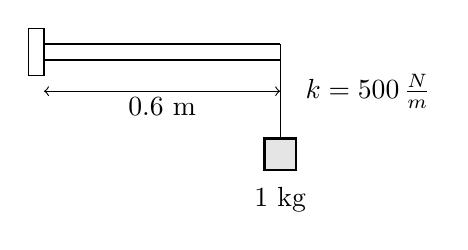
\begin{tikzpicture}
    % Draw the main beam
    \draw[thick] (0,0) -- (3,0);
    \draw[thick] (0,-0.2) -- (3,-0.2);
    
    % Add end support
    \draw (-0.2,-0.4) rectangle (0,0.2);
    
    % Add dimension line and label
    \draw[<->] (0,-0.6) -- (3,-0.6);
    \node at (1.5,-0.8) {0.6 m};
    
    % Draw spring
    \draw (3,0) -- (3, -1.2);
    \node[anchor=west] at (3.2, -0.6) {$k=500\,\frac{N}{m}$};
    
    % Draw mass
    \fill[gray!20] (2.8, -1.6) rectangle (3.2, -1.2);
    \draw[thick] (2.8, -1.6) rectangle (3.2, -1.2);
    \node[anchor=north] at (3, -1.7) {1 kg};
    
    \end{tikzpicture}



	    \begin{enumerate}
        \item $3.24$
        \item $20.36$
        \item $22.36$
        \item $3.56$
    \end{enumerate}

    \item A single degree of freedom system is vibrating with an initial \brak{\text{first cycle}} amplitude of $5 \text{ cm}$. The viscous damping factor associated with the vibrating system is $2\%$. The vibration amplitude of the fifth cycle \brak{\text{in cm}} is
    \begin{enumerate}
        \item $1.65$
        \item $4.41$
        \item $2.67$
        \item $3.02$
    \end{enumerate}

    \item A cruise missile with an ideal ramjet engine is flying at Mach $4.0$ at an altitude where the ambient temperature is $100 \text{ K}$. Consider the ratio of specific heats $\gamma = 1.4$ and specific gas constant $R = 287 \frac{J}{kg K}$. If the stagnation temperature in the combustion chamber is equal to $2310 \text{ K}$, the speed of the exhaust gases  is $\cdots$

    \item A gas turbine engine is operating under the following conditions:
    \begin{itemize}
        \item Stagnation temperature at turbine inlet: $1350 \text{ K}$
        \item Stagnation pressure at turbine inlet: $10 \text{ bar}$
        \item Static temperature at turbine exit: $800 \text{ K}$
        \item Velocity at turbine exit: $200  \frac{m}{s}$
        \item Total-to-total efficiency of turbine: $0.96$
        \item $\gamma$ \brak{\text{ratio of specific heats}}: $1.33$
        \item $C_p$ \brak{\text{specific heat at constant pressure}}: $1.147 \frac{ kJ}{kg K}$
    \end{itemize}
    
    The stagnation pressure \brak{\text{in bar}} in the nozzle \brak{\text{considering an isentropic nozzle}} is equal to $\dots$

    \item Air at a stagnation temperature of $300 \text{ K}$ $\brak{\text{ratio of specific heats}, \gamma = 1.4 }$and $\brak{\text{specific gas constant} R = 287 \frac {J}{kg K}}$ enters the impeller of a centrifugal compressor in axial direction. The stagnation pressure ratio between the diffuser outlet and impeller inlet is $4.0$. The impeller blade radius is $0.3 \text{ m}$ and it is rotating at $15000 \frac{ rev}{min}$. If the slip factor $\sigma$ ratio of tangential component of air velocity   at the blade tip to the blade tip speed is $0.88$, the overall efficiency \brak{\text{total-to-total}} of the compressor \brak{in \%} is

    \item A stationary two-stage rocket with an initial mass of $16000 \text{ kg}$, carrying a payload of $1000 \text{ kg}$, is fired in a vertical trajectory from the surface of the earth. Both stages of the rocket have the same specific impulse, $I_p$, of $300 \text{ s}$ and the same structural coefficient of $0.14$. The acceleration due to gravity is $9.8\frac{ m}{s^2}$. Neglecting drag and gravity effects and considering both stages with the same payload ratio, the terminal velocity attained by the payload in $\frac{m}{s}$ is

    \item An aircraft is flying at Mach $3.0$ at an altitude where the ambient pressure and temperature are $50 \text{ kPa}$ and $200 \text{ K}$, respectively. If the converging-diverging diffuser of the engine $\brak{\text{considered isentropic with a ratio of specific heats}, \gamma = 1.4}$ and $\brak{\text{specific gas constant} R = 287 \frac{ J}{kg K}}$ has a throat area of $0.05 \text{ m}^2$, the mass flow rate through the engine in $\frac{kg}{s}$ is
    \begin{enumerate}
        \item $197$
        \item $232$
        \item $790$
        \item $157$
    \end{enumerate}

    \item A cryogenic rocket has a specific impulse of $455 \text{ s}$ and a characteristic velocity of $2386 \frac{ m}{s}$. The value of the thrust coefficient for this rocket is
    \begin{enumerate}
        \item $1.78$
        \item $1.73$
        \item $1.87$
        \item $1.95$
    \end{enumerate}

    \item For a given airplane with a given wing loading executing a turn in the vertical plane, under what conditions will the turn radius be minimum and the turn rate be maximum?
    \begin{enumerate}
        \item Highest possible $C_L$ and lowest possible load factor
        \item Lowest possible $C_L$ and lowest possible load factor
        \item Lowest possible $C_L$ and highest possible load factor
        \item Highest possible $C_L$ and highest possible load factor
    \end{enumerate}

    \item Lift-off distance for a given aircraft of weight $W$ is $S_{\text{LO}}$. If the take-off weight is reduced by $10\%$, then the magnitude of percentage change in the lift-off distance \brak{\text{assuming all other parameters to remain constant}} is


 






 


